% \section{Introdução}

% O Brasil possui uma extensa costa de 8{,}7 mil quilômetros, com 68 portos e uma faixa litorânea que concentra mais da metade da população e do PIB do país. Além disso, o país possui aproximadamente 4{,}5 milhões de quilômetros quadrados de águas jurisdicionais, onde se encontram recursos estratégicos como 95\% do petróleo e 83\% do gás natural nacionais, e por onde transitam cerca de 95\% do comércio exterior \cite{andrade_2021}.
% Nesse contexto, a crescente adoção de Veículos Aéreos Não Tripulados (VANTs) em operações de vigilância marítima exige métodos mais robustos de planejamento de rotas, especialmente em cenários com alvos parcialmente conhecidos e detecção sensorial sujeita a limitações práticas. Trabalhos anteriores mostram que a vigilância baseada em varredura aérea pode ser modelada como uma variação do Problema do Caixeiro Viajante (TSP), incorporando restrições operacionais como autonomia limitada, sensores com alcances distintos e alvos móveis ou parcialmente observáveis \cite{marlow_2007}.
% Técnicas de otimização como o \textit{Simulated Annealing} têm se mostrado eficazes em problemas de roteamento com grande espaço de busca e múltiplos mínimos locais, sendo uma escolha promissora para o replanejamento progressivo de trajetos em ambientes com inserção dinâmica de alvos \cite{kosmas_2012}.
% Mais recentemente, abordagens com replanejamento dinâmico em tempo real vêm sendo propostas para garantir a cobertura de alvos não detectados ou mal inspecionados, especialmente em aplicações com VANTs e sensores embarcados \cite{penicka_2017}. Motivado por esses avanços, este trabalho propõe uma formulação adaptada do TSP para missões de patrulha marítima com inserção condicional de novos alvos, levando em conta restrições de distância lateral, autonomia do VANT e alcance heterogêneo de sensores.


\section{Introdução}

O uso de Veículos Aéreos Não Tripulados (VANTs) em operações de vigilância marítima tem se expandido significativamente, impulsionado por desafios associados à extensão da costa brasileira e à importância estratégica de suas águas jurisdicionais, que concentram a maior parte do comércio exterior e das reservas nacionais de petróleo e gás natural \cite{andrade_2021}. Esses cenários exigem métodos eficientes de planejamento de rotas, sobretudo quando os alvos são parcialmente conhecidos e os sensores têm capacidades limitadas.

A tarefa pode ser modelada como uma variação do Problema do Caixeiro Viajante (TSP), incorporando restrições operacionais como autonomia limitada, sensores de diferentes alcances e alvos móveis ou parcialmente observáveis \cite{marlow_2007}. Técnicas como o \textit{Simulated Annealing} têm mostrado bom desempenho em problemas de roteamento com múltiplos mínimos locais, sendo úteis para o replanejamento dinâmico \cite{kosmas_2012}. Abordagens mais recentes propõem replanejamento em tempo real com base em dados sensoriais para garantir cobertura progressiva de alvos não detectados \cite{penicka_2017}.

Este trabalho propõe uma abordagem baseada em TSP adaptado para patrulha marítima com inserção progressiva de novos alvos detectados durante a missão, respeitando as limitações operacionais do VANT e explorando estratégias de navegação dinâmicas.

\begin{figure}[H]
    \centering
    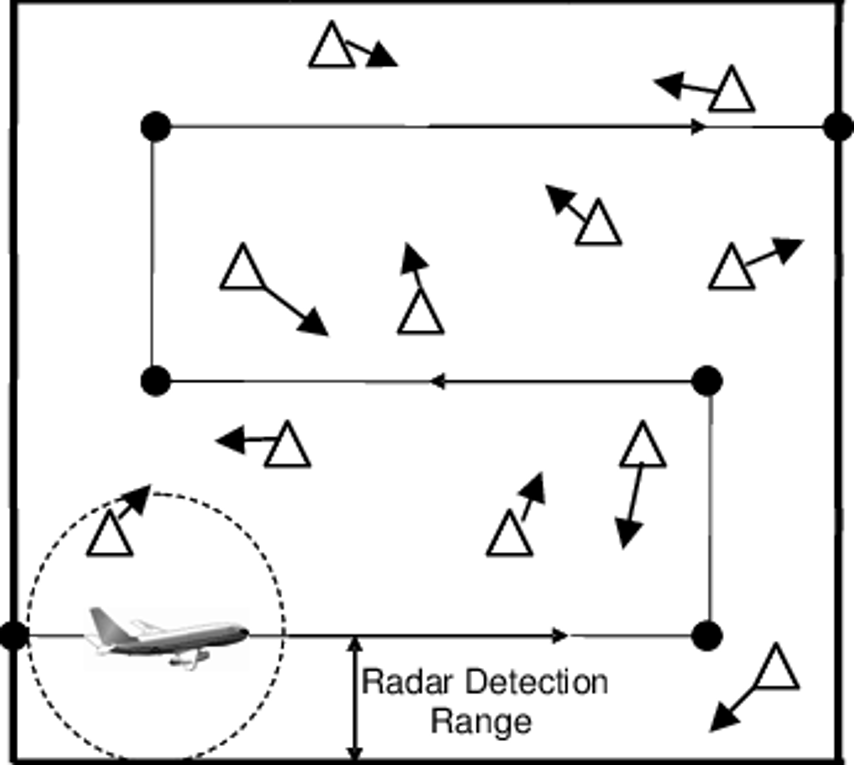
\includegraphics[width=0.5\textwidth]{fig/vant.png}
    \caption{Patrulha naval realizada por aeronave.}
    \small
    \textbf{Fonte:} \cite{marlow_2007}.
\end{figure}
